\chapter{Local Motor Invariant}

\ifpdf
    \graphicspath{{LocalInvariant/LocalInvariantFigs/PNG/}{LocalInvariant/LocalInvariantFigs/PDF/}{LocalInvariant/LocalInvariantFigs/}}
\else
    \graphicspath{{LocalInvariant/LocalInvariantFigs/EPS/}{LocalInvariant/LocalInvariantFigs/}}
\fi

\section{Introduction}
Global Motor Invariant keeps the topology motion primitives.
For animal motion is also of high accuracy.
In this chapter we focus on the control on the quantitative properties of motion.
In our research, we try to limit the computational cost.


The discovery is that motion of natural system will change in a uniform way.
The method we proposed exploring the symmetry properties of dynamics system.
The symmetry property of a dynamic system is called local motor invariant.
The method we propose is based the lie group theory.

\subsection{Group and Symmetry}
Symmetry in geometrical sense means when you transform an shape, the transform one and original one are exactly the same.
For the square examples, rotation it by 90 degree will make it exactly the same with the original one.



\begin{figure}[!htbp]
  \begin{center}
    \leavevmode
    \ifpdf
      \includegraphics[height=6in]{Symmetry}
    \else
      \includegraphics[width=0.7\textwidth]{Symmetry}
    \fi
    \caption{Symmetry}
    \label{fig:symmetry}
\end{center}
\end{figure}
All the action that can preserve the symmetry is defined as the set as group.
A group has the following properties.
If g1 ,g2 in G
g1*g2 in G
g1 *g2=e;

In algebra, a shape can implicitly defined by an function I(x)=0;
The group transformation is define by x’=g(x)
If symmetry is met, we have I(x)=I(g(x)).
We can say I(x) is an invariant function of group G.

We have to note that f(x) is not only the shape unchanged by g.
In fact ,many shape is invariant, and form a space, the invariant space.
In fact, we can pick up and two shape and combination is also an invariant shape. 


\begin{figure}[!htbp]
  \begin{center}
    \leavevmode
    \ifpdf
      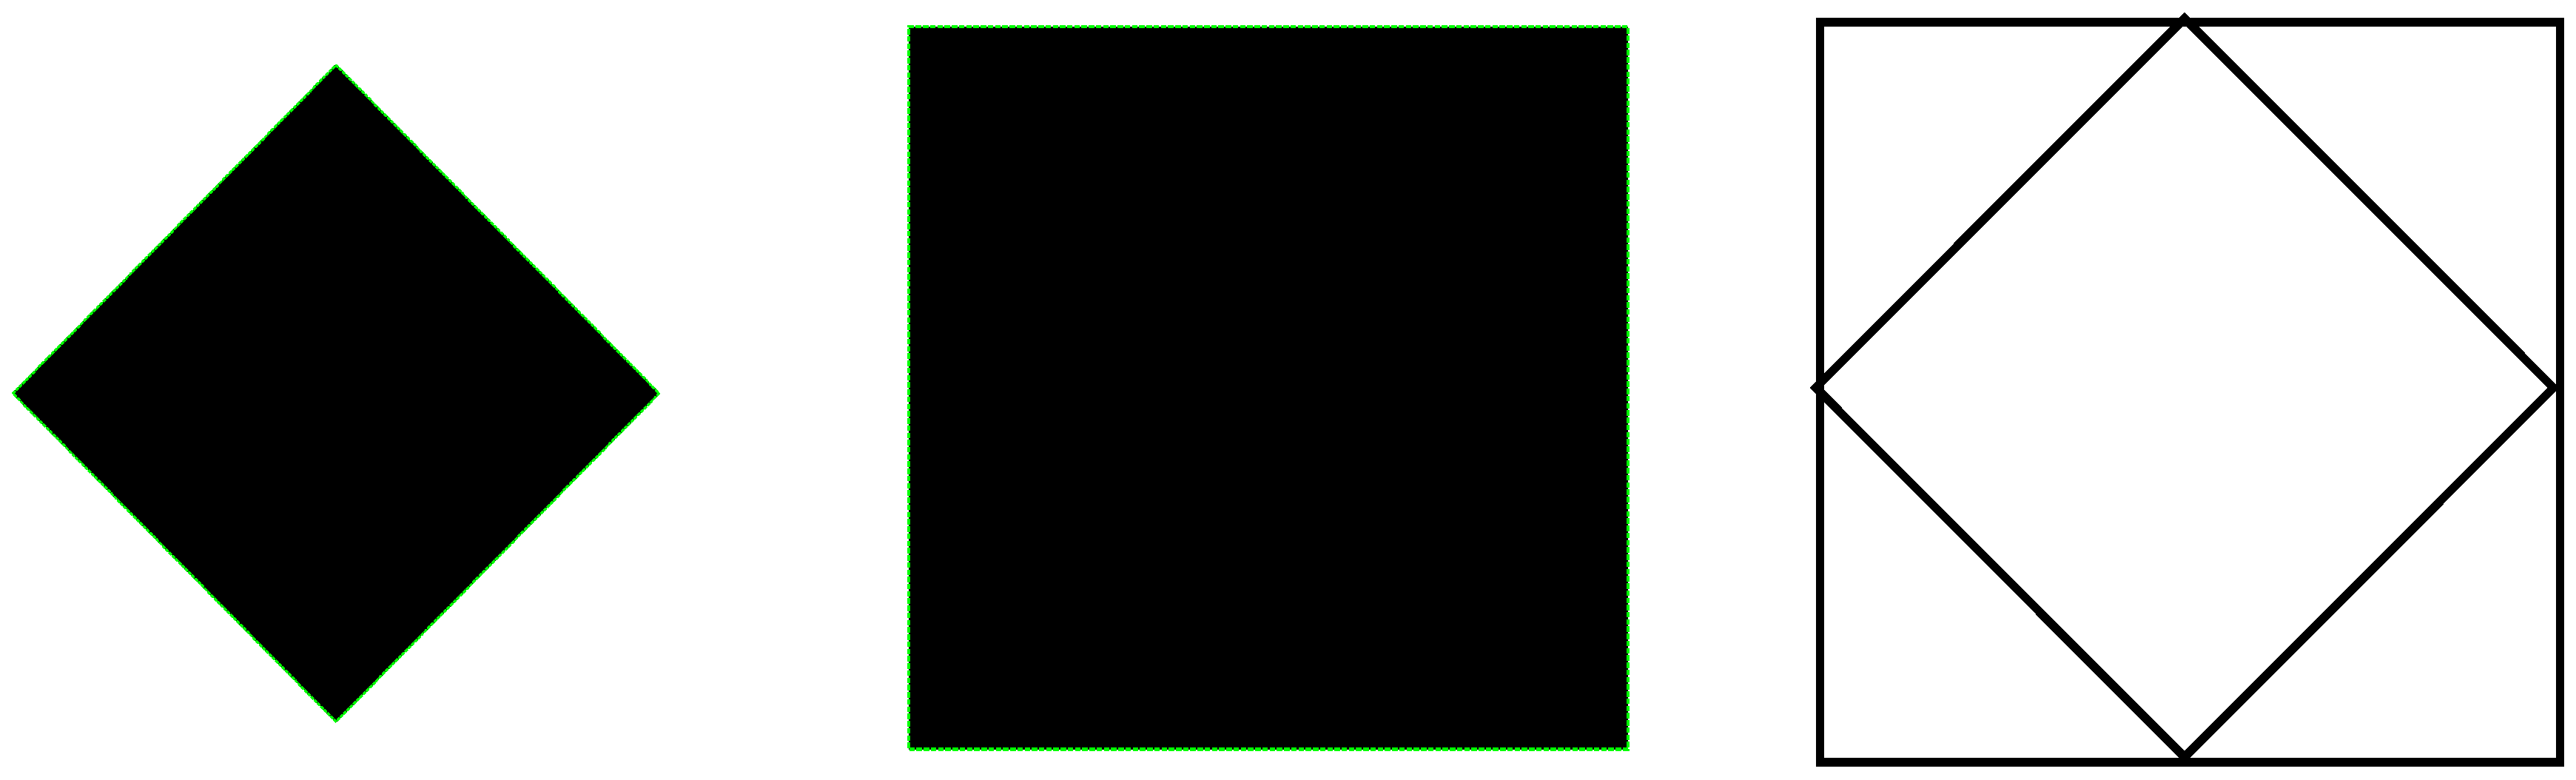
\includegraphics[height=6in]{SymmetrySpace}
    \else
      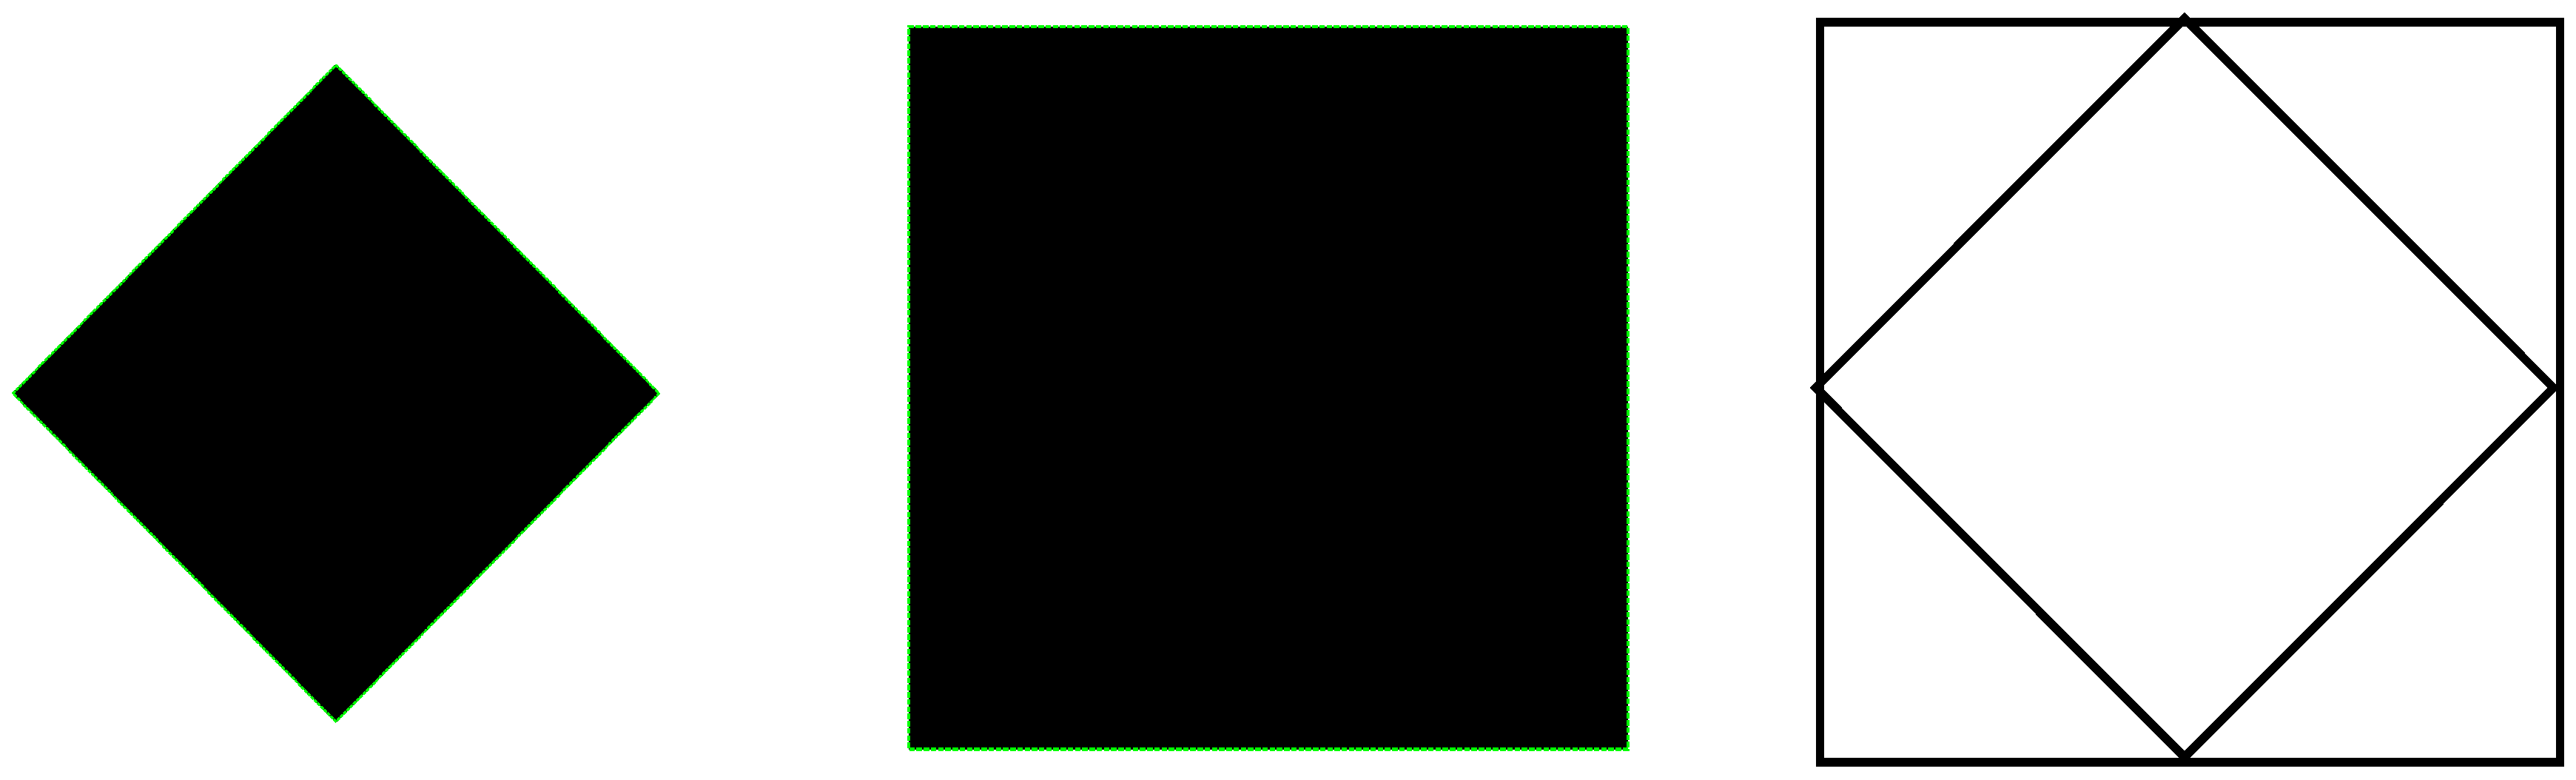
\includegraphics[width=0.7\textwidth]{SymmetrySpace}
    \fi
    \caption{Symmetry}
    \label{fig:symmetry}
\end{center}
\end{figure}





\subsection{Lie Group and Symmetry of Dynamic System}
Lie Group is continues group original from study of differential equation.
For Physically-based animation,
Motion is usually described by the differential equation (1)
\begin{equation}
	\dot{X}=F(x,u)
\end{equation}
Physically possible motion is the solution of the equation.
An important property from one solution x, with a group action g, we ca get another solution $x_a$
 	\[
x_a=g_a(x)
\]
.
for example
, 
We have 

So the group action is


For equation (1), the group action $g_a$ satisfy the symmetry property (2).
	(3)
This provide us an idea about motion synthesis.
Given an original motion m, and the corresponding group g, a new motion is generated by g(m).

For every group G, we can find an function I(x) unchanged by the group action G, 

I(x) are called local motion invariant. 
For mechanical system,  I(x) has important physically meaning. 
I(x) corresponding to the Conservative Law like energy or angular momentum.
\section{Controlled Symmetry}

For motion synthesis, usually the desired motion is ma
For example for motio stability, we want the current state is within the basin of attraction.
If we want to control the final motion style, we want the state is on the limit cycle.

For motion sysnthesis, the problem is given the system, let the original system have the desired symmetry.

 and original motion m is  known, but the corresponding group action $g_a$ is not satisfied by differential equation.
For such situation, control input u  is added, which modify the original equation to allow the designed G, this is called Controlled Symmetry.

Most dynamic motion can be modelled as an Lagrange System. 
\[
L=K(\dot(q)-V(q).
\]
And the desired action G must keep the L invariant. 

The original m is defined by the eural langrage equation
\begin{equation}
\frac{d}{dt} \frac{\partial L}{\partial \qd} - \frac{\partial L}{\partial q} = 0
\label{eq:uncontrolled_euler_lagrange}
\end{equation}
The modified system is 
\begin{align}
\frac{d}{dt} \frac{\partial L}{\partial Tg(\qd)} - \frac{\partial L}{\partial g(q)}&=0,\label{eq:liegroup_euler_lagrange}\\
\frac{d}{dt} \frac{\partial L}{\partial \qd} - \frac{\partial L}{\partial q}&=\ulocal. \label{eq:controlled_euler_lagrange}
\end{align}


(5) and (6) are the equivalent equation, by comparing  equation (5) and (6), we can get u
Some Specific example of Symmetry and Control
\subsection*{ Offset Action}
\[
\goff(q) = q+r
\]
Which keep speed, but modify the pos. thus keep the K but modify V

\begin{equation}
\ulocal(\x) = \frac{\partial}{\partial q} \left(V(\goff(q)) - V(q)\right).
\end{equation}

\begin{figure}[!htbp]
  \begin{center}
    \leavevmode
    \ifpdf
      \includegraphics[height=6in]{g_off}
    \else
      \includegraphics[width=0.7\textwidth]{g_off}
    \fi
    \caption{Offset Action}
    \label{fig:goff}
\end{center}
\end{figure}
on phase space, if q is the horizontal axis, and $\dot{q}$ is the vertical axis, this has the effect of moving the phase plot right and right.
\subsection*{Time Scalling}

%g_st(q,dot{q})=(q,st*dot{q})
we have
$T\gts(\qd)=\alpha \qd$
\begin{equation}
\ulocal(\x) = (\alpha^2 - 1) \frac{\partial V(q)}{\partial q}.
\end{equation}

\begin{figure}[!htbp]
  \begin{center}
    \leavevmode
    \ifpdf
      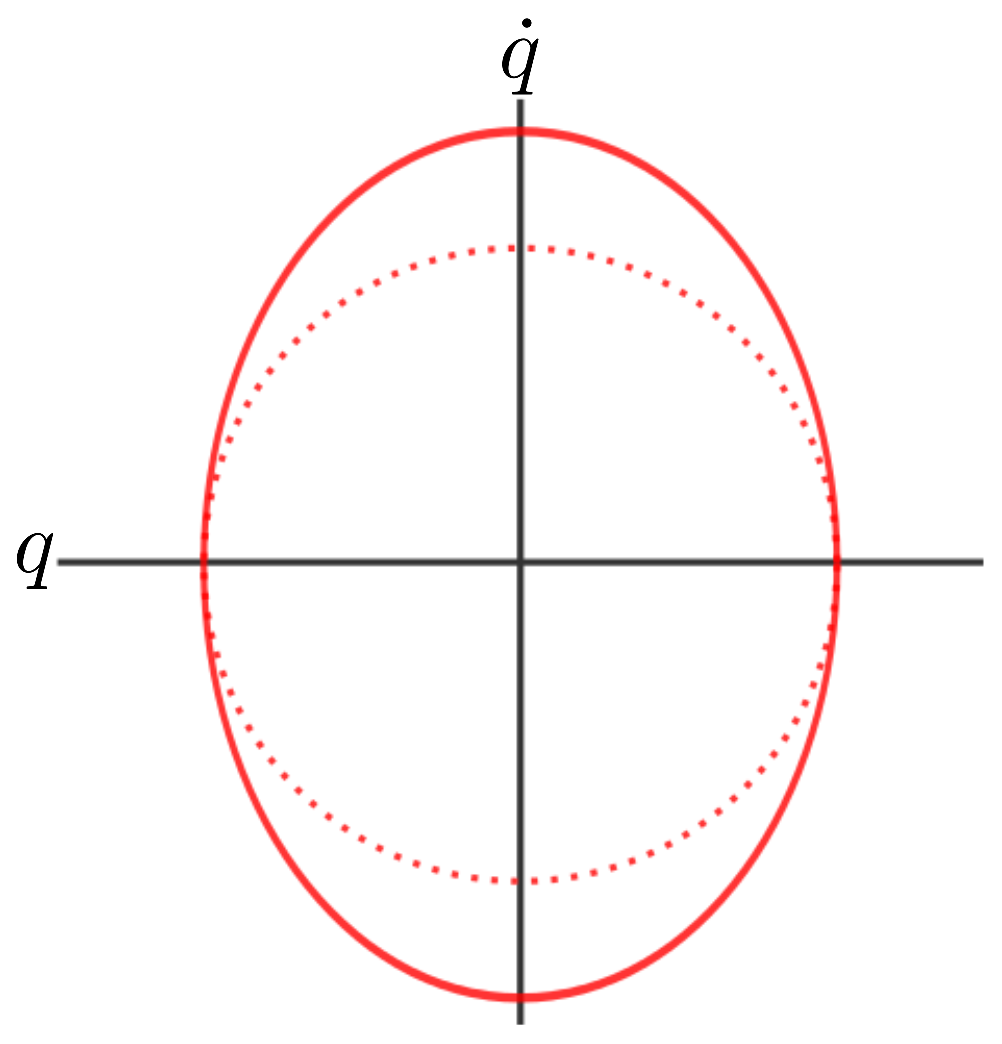
\includegraphics[height=6in]{g_ts}
    \else
      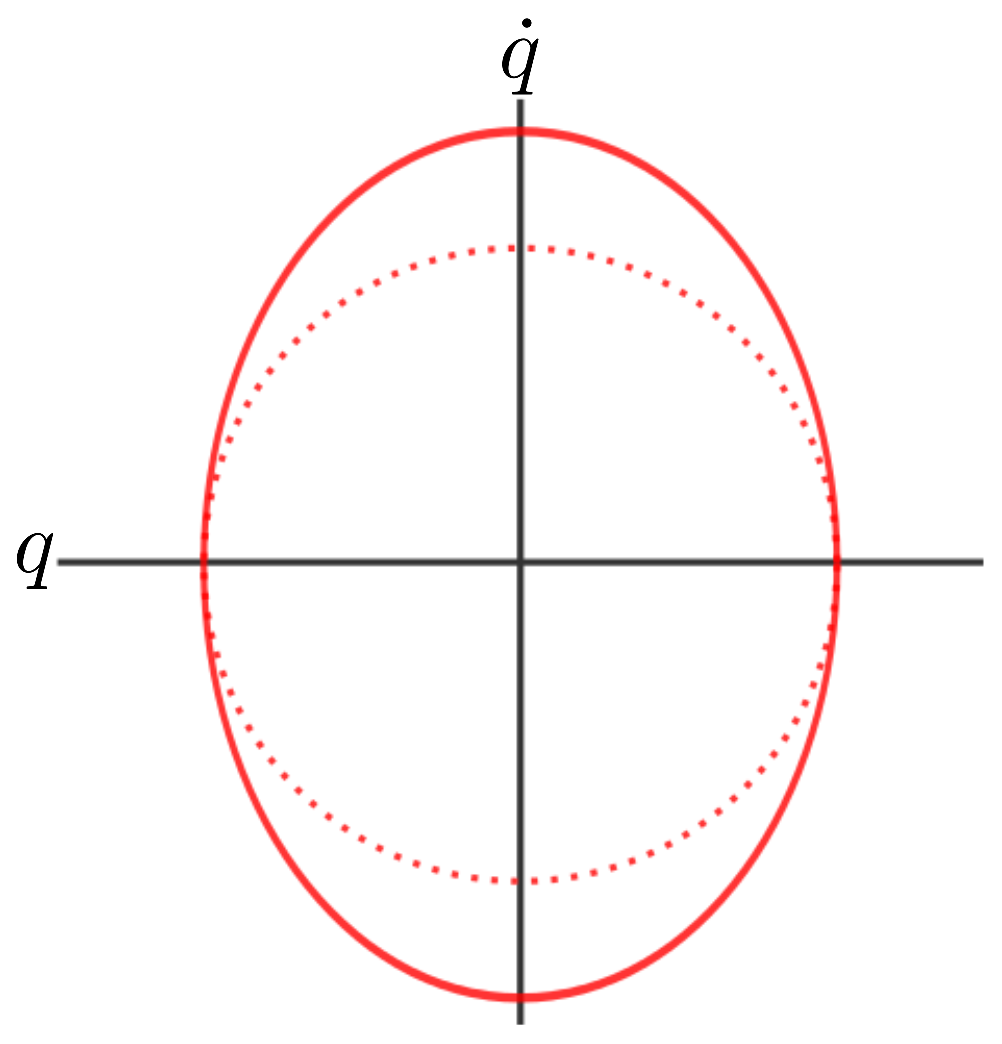
\includegraphics[width=0.7\textwidth]{g_ts}
    \fi
    \caption{Time Scaling Action}
    \label{fig:gts}
\end{center}
\end{figure}
on phase space, this has the effect strength the phase plot in the vertical direction

\subsection*{energy scaling}
For some system moving the the conservtime field with constant mass matrix.
The energy is preserved and different motion present different level of energy.
For such system, we have the 
For such

%g_e(q,\dot{q})=(e^2*q,e*\dot{q}).
U can be developed by applying the pos scaling and time scaling in a combined manner.

On phase plot, this has the effect enlarge the phase portrait.

\begin{figure}[!htbp]
  \begin{center}
    \leavevmode
    \ifpdf
      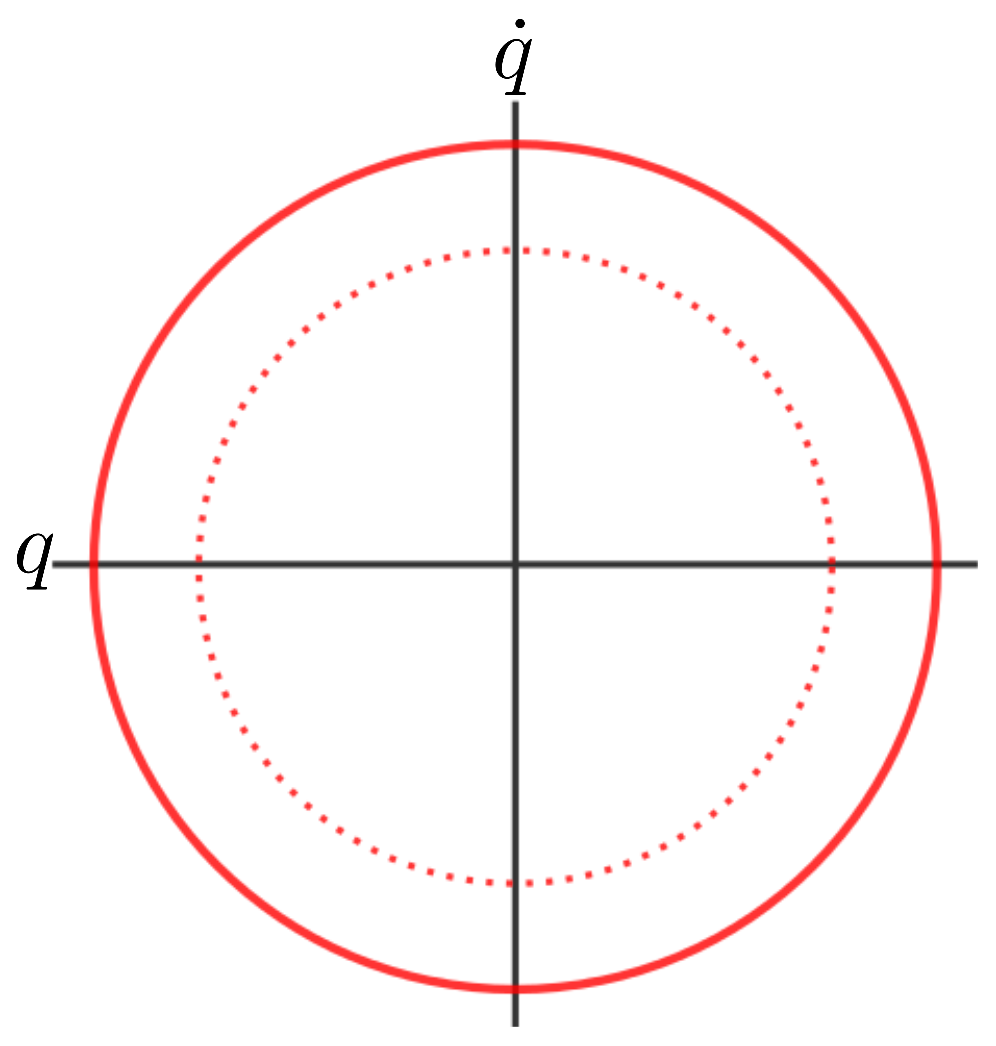
\includegraphics[height=6in]{g_en}
    \else
      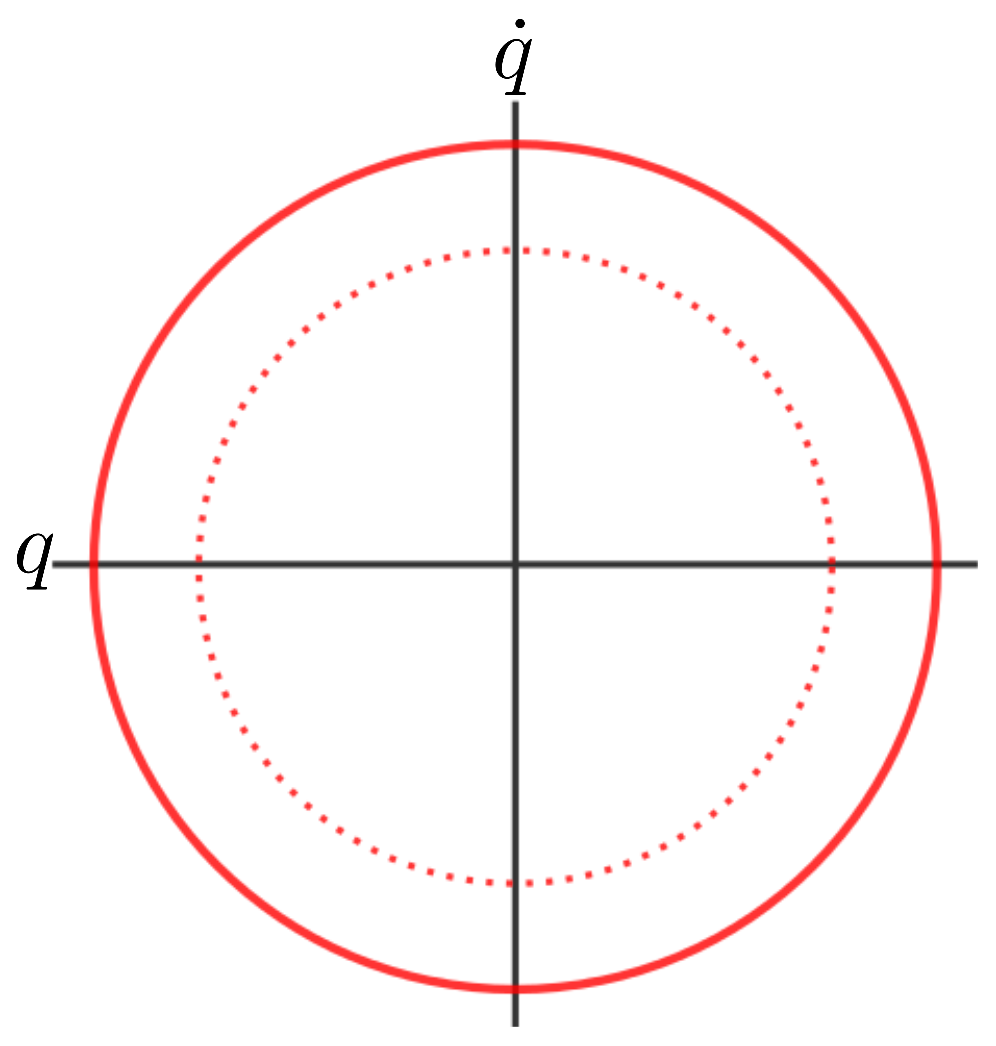
\includegraphics[width=0.7\textwidth]{g_en}
    \fi
    \caption{Energe Scaling Action}
    \label{fig:gen}
\end{center}
\end{figure}
\subsection*{time offset}
Is q(t) is solution to f(q)

%g_{toff}(q(t) \dot{q}(t))=(q(t+toff),\dot{q}(t+toff))
For dynamic system, this seems obvious. And no control is need for such symmetry.
For system with limit circle, this $g_toff$ has a special effects like phase modification.

On phase plot, this has the effect rotate on the limit circle about an angle.


\begin{figure}[!htbp]
  \begin{center}
    \leavevmode
    \ifpdf
      \includegraphics[height=6in]{g_off}
    \else
      \includegraphics[width=0.7\textwidth]{g_off}
    \fi
    \caption{Offset Action}
    \label{fig:goff}
\end{center}
\end{figure}





\section{Simple Example}
Bouncing Ball
The bouncing ball system has a energy scaling symmetry, if bouncing height is q(t), $\dot{q(t)}$
The new system is 
%Eq(t) \dot{e^2q{t}}

as show in figure

\begin{figure}[!htbp]
  \begin{center}
    \leavevmode
    \ifpdf
      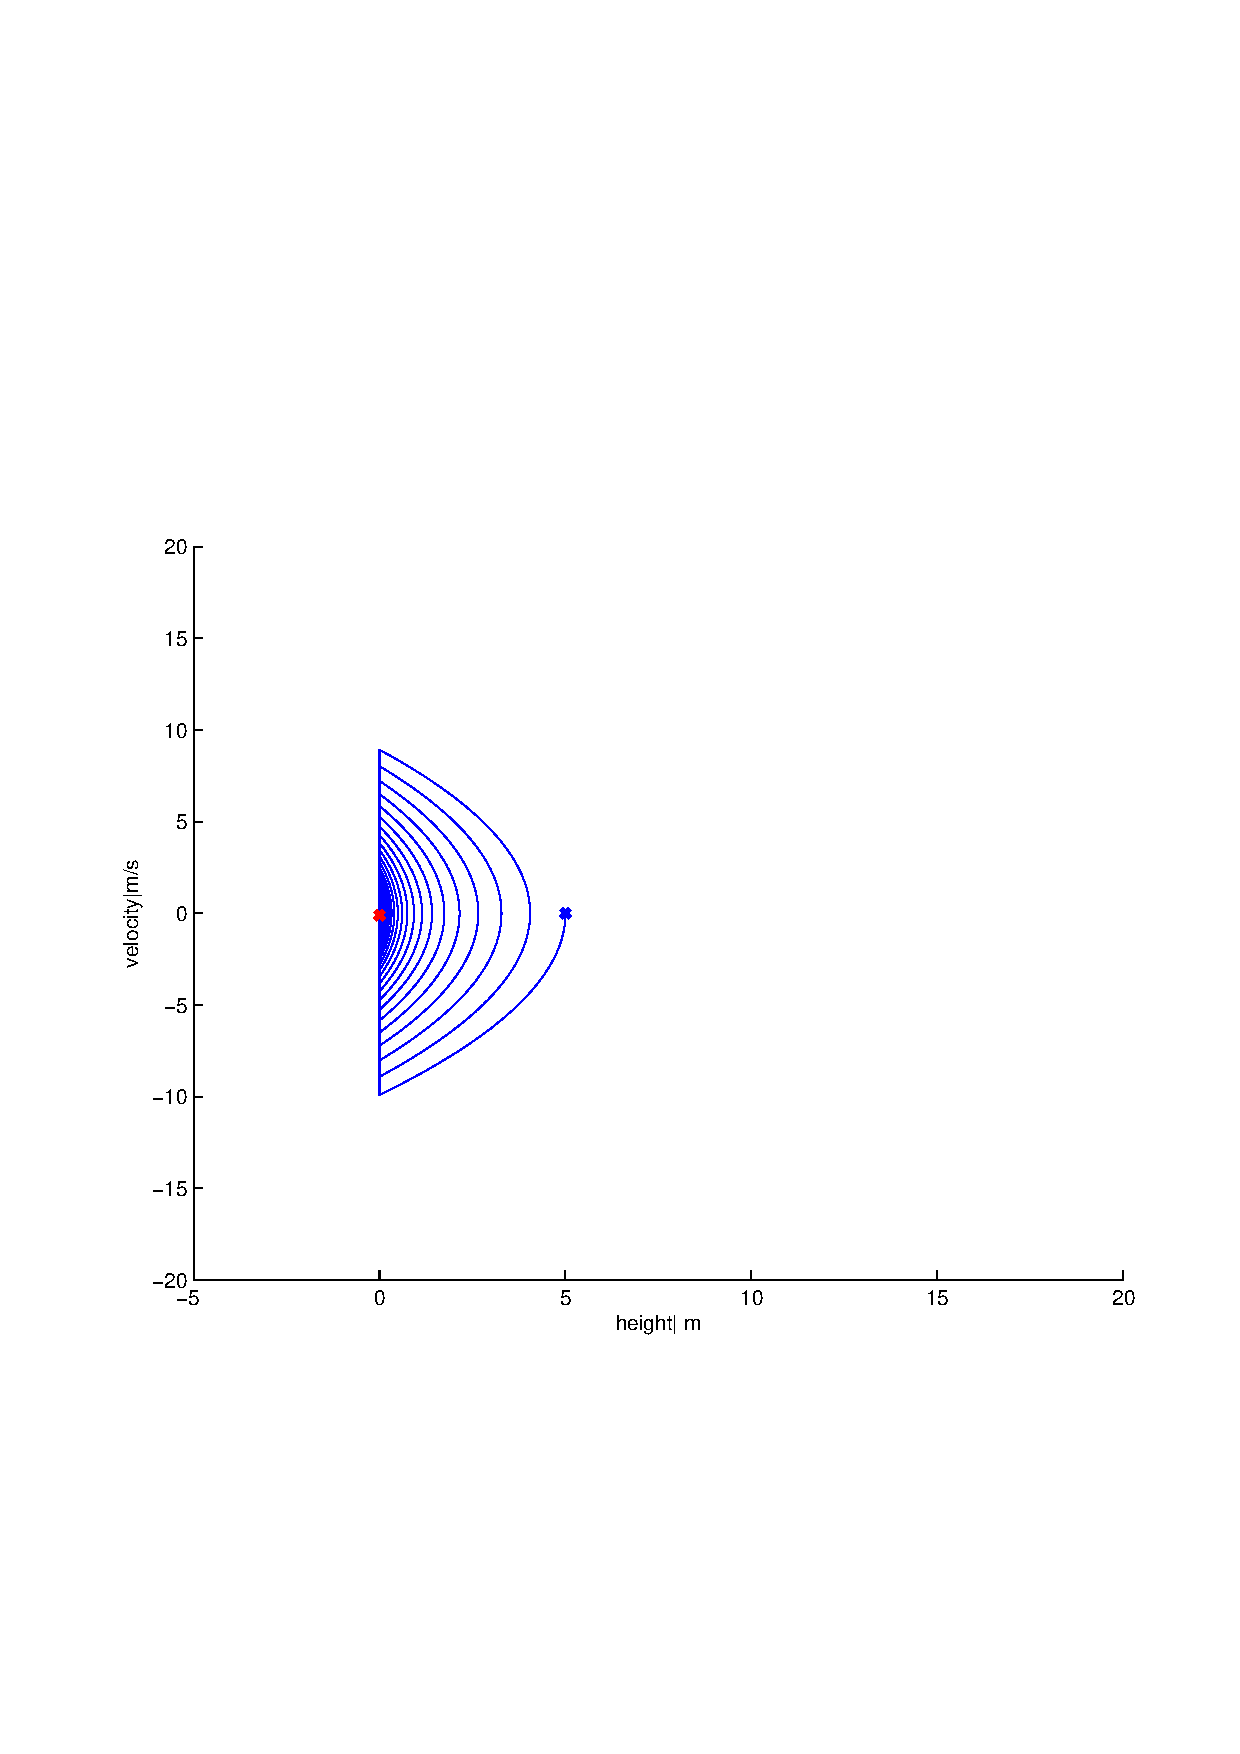
\includegraphics[height=6in]{BouncingBallPhasePlotuncontrolledDropAt5}
    \else
      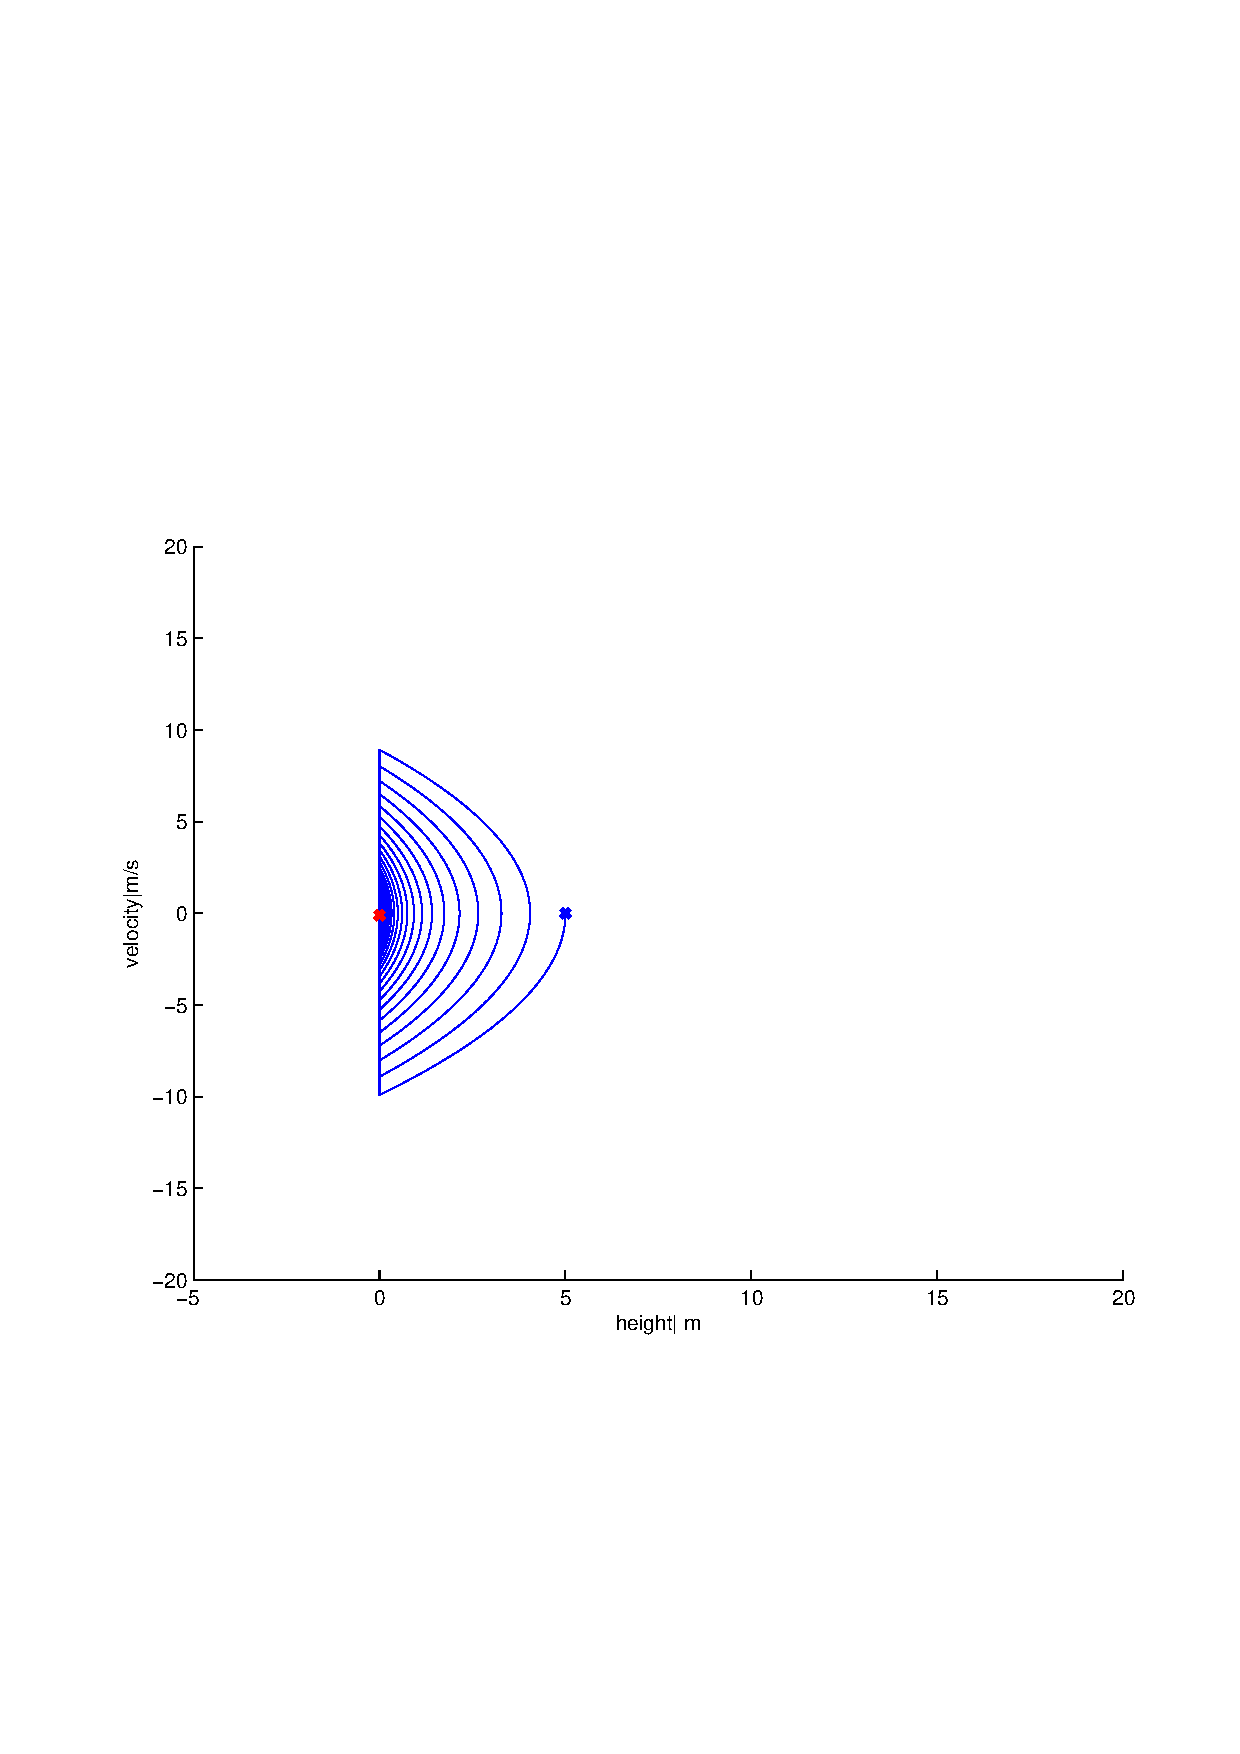
\includegraphics[width=0.7\textwidth]{BouncingBallPhasePlotuncontrolledDropAt5}
    \fi
    \caption{Drop at Filen}
    \label{fig:bouncing5}
\end{center}
\end{figure}


\begin{figure}[!htbp]
  \begin{center}
    \leavevmode
    \ifpdf
      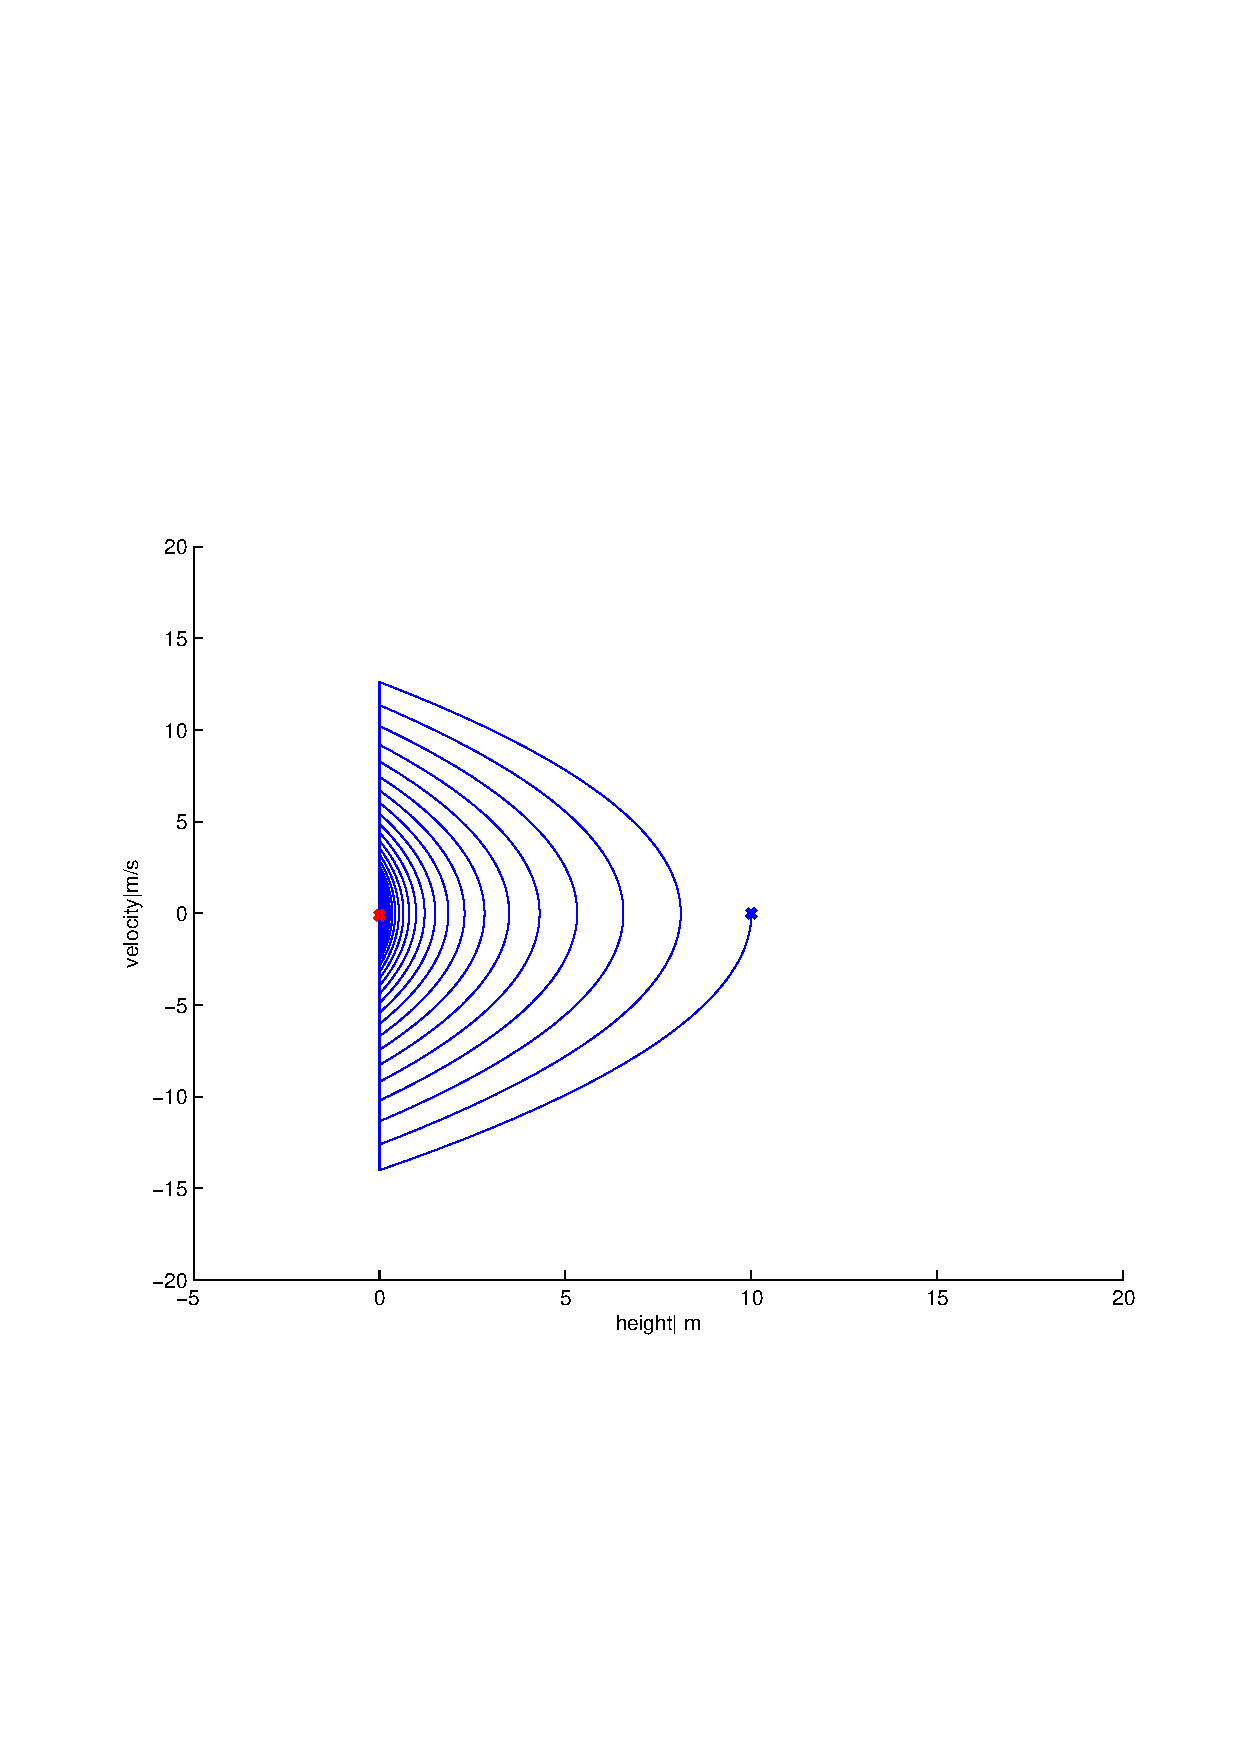
\includegraphics[height=6in]{BouncingBallPhasePlotuncontrolledDropAt10}
    \else
      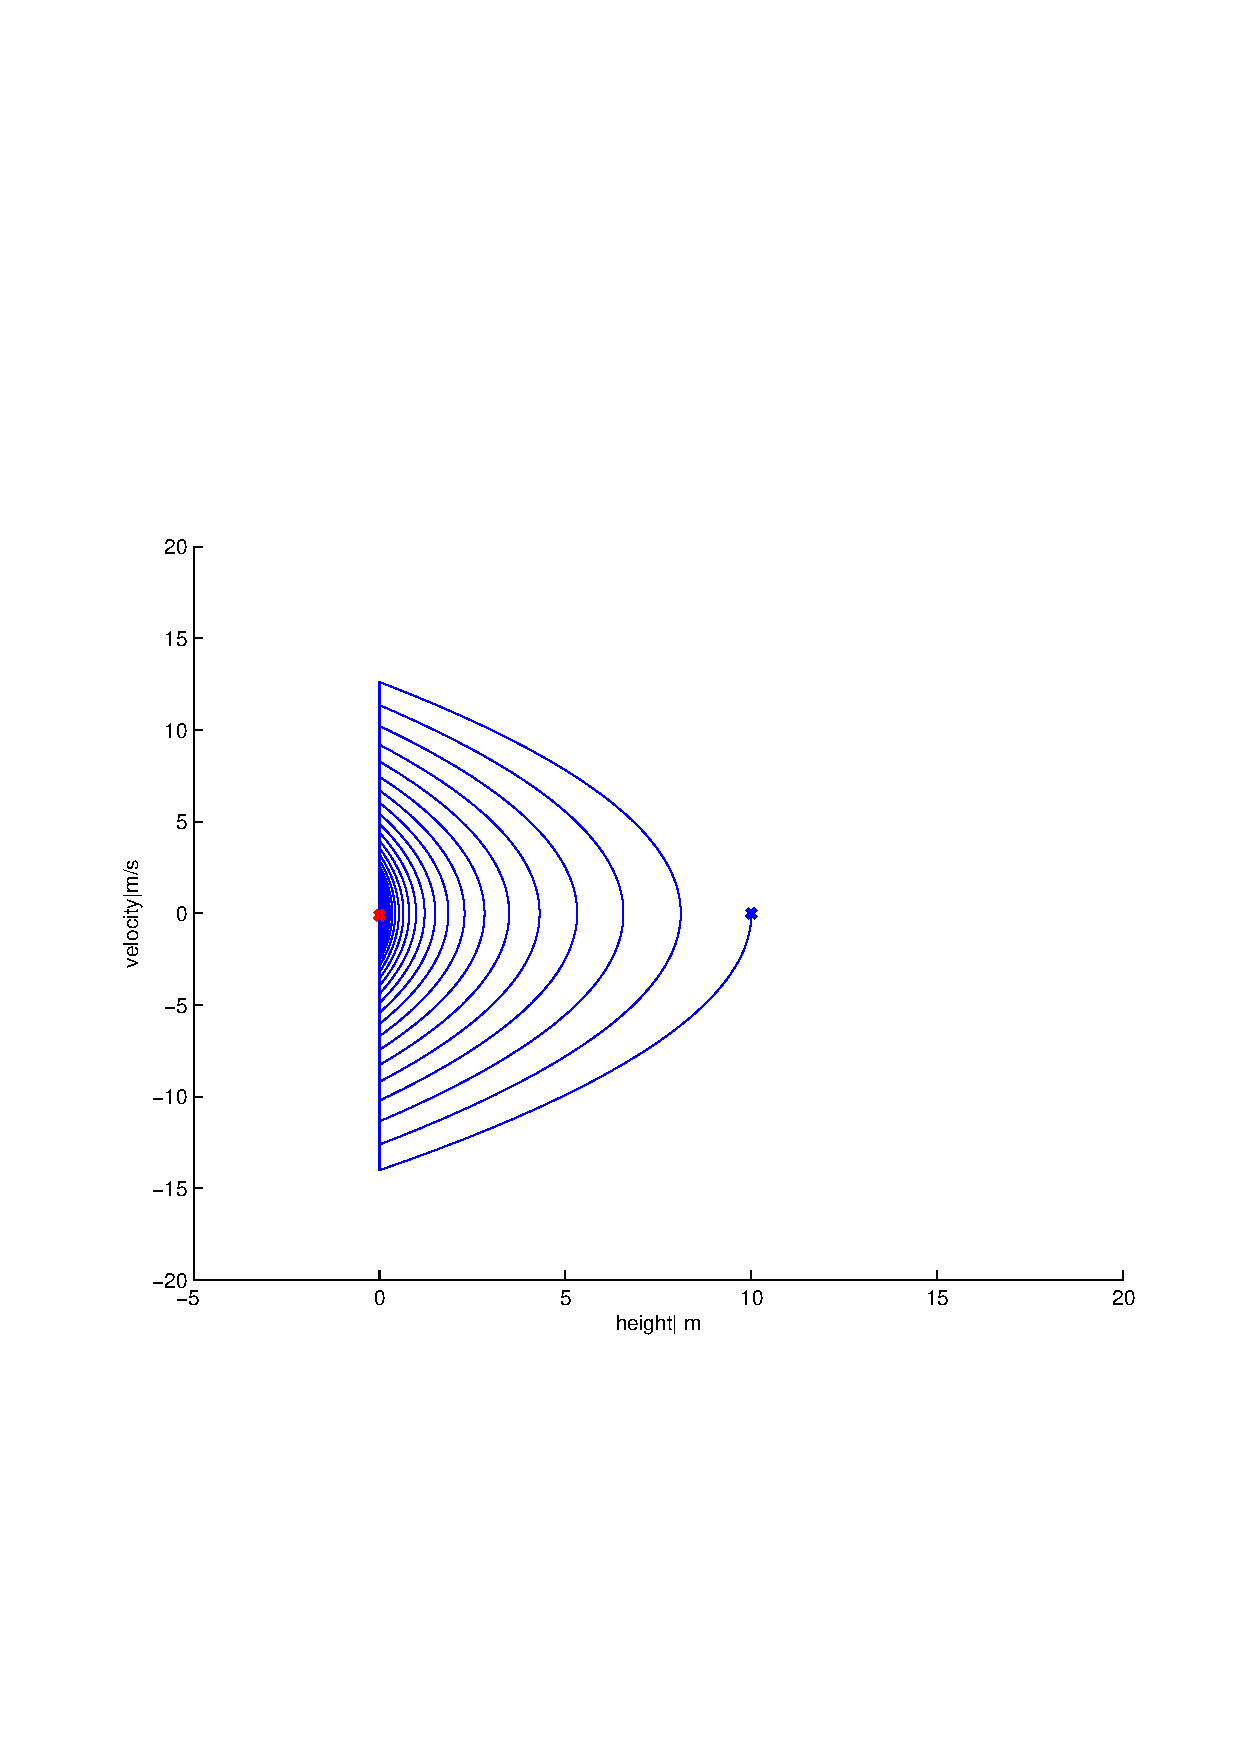
\includegraphics[width=0.7\textwidth]{BouncingBallPhasePlotuncontrolledDropAt10}
    \fi
    \caption{Drop at 10}
    \label{fig:bouncing5}
\end{center}
\end{figure}
